\documentclass[a0]{a0poster}
% You might find the 'draft' option to a0 poster useful if you have
% lots of graphics, because they can take some time to process and
% display. (\documentclass[a0,draft]{a0poster})

\pagestyle{empty} %no header, footer,  nor page numbers
\setcounter{secnumdepth}{0} %create counter
\setlength\paperheight{36in} \setlength\paperwidth{48in} %set poster size
\setlength\textwidth{\paperwidth} %give names to poster width
\setlength\textheight{\paperheight} %give names to poster height

% The textpos package is necessary to position textblocks at arbitary
% places on the page.
\usepackage[overlay,absolute]{textpos}
\usepackage[justification=centering]{caption}
% Graphics to include graphics. Times is nice on posters, but you
% might want to switch it off and go for CMR fonts.
\usepackage{graphicx}
\usepackage{amsmath}
\usepackage{color}
\usepackage{wallpaper}
\usepackage{tikz}
\usepackage{url}
\usepackage{colortbl}
\usepackage{multirow,bigdelim}
\usepackage{arydshln}
\usepackage{booktabs}
\usepackage{caption, subcaption}
\usepackage{amssymb}
\usepackage{epstopdf}
\usepackage{float}
\usepackage{enumerate}
\usepackage{pgfplots}
\usepackage{etex}
\usepackage{MnSymbol,wasysym}
\usepackage{cite}
\usepackage{verbatim}
\usepackage[justification=centering]{caption} 
\captionsetup{justification=centering}

\usetikzlibrary{patterns}



\definecolor{DarkBlue}{rgb}{0.1,0.1,0.5}
\definecolor{dollarbill}{rgb}{0.52, 0.73, 0.4}
\definecolor{teagreen}{rgb}{0.82, 0.94, 0.75}


\definecolor{carolinablue}{rgb}{0.6, 0.73, 0.89}
\definecolor{non-photoblue}{rgb}{0.64, 0.87, 0.93}
\definecolor{powderblue(web)}{rgb}{0.69, 0.88, 0.9}
\definecolor{beaublue}{rgb}{0.74, 0.83, 0.9}
\definecolor{byzantium}{rgb}{0.44,0.16,0.39}
\definecolor{columbiablue}{rgb}{0.61, 0.87, 1.0}
\definecolor{coolblack}{rgb}{0.0, 0.18, 0.39}
\definecolor{deepjunglegreen}{rgb}{0.0, 0.29, 0.29}
\definecolor{junglegreen}{rgb}{0.16, 0.67, 0.53}
\definecolor{mangotango}{rgb}{1.0, 0.51, 0.26}
\definecolor{steelblue}{rgb}{0.27, 0.51, 0.71}




%\definecolor{background}{RGB}{176,213,255}
\definecolor{white}{RGB}{255,255,255}
\definecolor{black}{rgb}{0.0, 0.0, 0.0}
%\pagecolor{background}



\color{black}



\newcommand{\smallspace}{\vspace{2mm}}
\newcommand{\ds}{\displaystyle}
% see documentation for a0poster class for the size options here
\let\Textsize\normalsize


\def\LHead#1{\colorbox{deepjunglegreen}{\noindent{\textbf{\Huge\color{white} #1}}\bigskip}}
\def\Title#1{\noindent{\textbf{\VeryHuge\color{deepjunglegreen} #1}}}
\def\Subtitle#1{\noindent{\textbf{\Huge\color{deepjunglegreen} #1}}}





\begin{document}


\TPGrid[1.5in,1.5in]{45}{33}      % margins 1.5in all around

\parindent=0pt
\parskip=0.5\baselineskip





\begin{textblock}{5}(0,0)
\includegraphics[scale=.15]{ValpoLogo.jpg}
\end{textblock}
\begin{textblock}{5}(41.75,0)
\includegraphics[scale=.75]{NSFlogo.png}
\end{textblock}



\begin{textblock}{32}(6.45,.3)
\begin{center}
\Title{\\ Noise-Induced Stabilization of Hamiltonian Systems}\\ 
%\vspace{30pt} Hamiltonian Systems}\\
\vspace{85pt}
\Subtitle{Anthony Coniglio, Sarah Sparks, Dan Weithers, Advisor: Dr.~Tiffany Kolba}

\end{center}
\end{textblock}

\begin{textblock}{45.5}(-0.25,4)
\hspace{0in}
\hrule
\end{textblock}
    


\begin{textblock}{11.5}(-0.25,4)
\medskip
\LHead{\parbox{11.5in}{\begin{center}Introduction\end{center}}}\\  %*1*
\large
\qquad\\
A \textbf{Hamiltonian system} is a two-dimensional system of differential equations defined by a Hamiltonian function $H(x,y)$ given by:
\begin{align*}
\frac{dX_t}{dt} &= \frac{\partial H}{\partial y}(X_t,Y_t) \\
\frac{dY_t}{dt} &= -\frac{\partial H}{\partial x}(X_t,Y_t)
\end{align*}
\begin{itemize}
\item The value of the Hamiltonian function $H(x,y)$ is constant along any solution curve
\end{itemize}
\qquad\\

\begin{textblock}{11.5}(-0.25,10.8)
\hspace{0in}
\hrule
\end{textblock}

We say that a system is \textbf{stable} if it is stochastically bounded; i.e. for all initial conditions and all $\delta>0$, there exists some bound $M$ such that
$$P(|(X_t, Y_t)|\leq M)>1-\delta$$
for all $t\geq0$.\\
\begin{itemize}
\item This definition reduces to boundedness in the deterministic setting
\end{itemize}
\medskip
\qquad\\
\end{textblock}

\begin{textblock}{11.5}(-0.25,16)
\medskip
\LHead{\parbox{11.5in}{\begin{center}Our Problem\end{center}}}\\  %*1*
\large
\qquad\\
\textbf{Noise-Induced Stabilization} is the phenomenon that occurs when the addition of randomness to an unstable system of ordinary differential equations results in a stable system of stochastic differential equations (SDEs).

\begin{itemize}
\item Unstable Hamiltonian systems cannot be stabilized by the addition of noise that is constant in space
\end{itemize}
\qquad\\

\begin{textblock}{11.5}(-0.25,21.8)
\hspace{0in}
\hrule
\end{textblock}

\textbf{Our Focus:}\\
Given an unstable Hamiltonian system, find a way to deterministically perturb the system so that:
\begin{itemize}
\item The qualitative behavior of the perturbed system is fundamentally the same as the original Hamiltonian system
\item The perturbed system exhibits noise-induced stabilization
\end{itemize}
\qquad\\

\begin{textblock}{11.5}(-0.25,26.6)
\hspace{0in}
\hrule
\end{textblock}

A \textbf{perturbed Hamiltonian system with noise} will have the following form:
\begin{align*}
\frac{dX_t}{dt} &= \frac{\partial H}{\partial y}(X_t,Y_t) - f(X_t,Y_t) + \epsilon_1 \frac{dB_1}{dt}\\
\frac{dY_t}{dt} &= -\frac{\partial H}{\partial x}(X_t,Y_t) - g(X_t,Y_t) + \epsilon_2 \frac{dB_2}{dt}
\end{align*}

\begin{itemize}
\item Functions $f$ and $g$ are the deterministic perturbations of the system
\item $B_1$ and $B_2$ are independent Brownian motions
\item $\epsilon_1$ and $\epsilon_2$ are constants that control the strength of the noise
\end{itemize}

\end{textblock}



%%%%%%%%%%%%%%%%%%%%%%%%%%%%%%%%%%%%%%%%%%%%%%%%%%%%%%%%%%%%%%%%%




\begin{textblock}{21.5}(11.75,4)
\medskip
\LHead{\parbox{21.5in}{\begin{center}Theorems\end{center}}}\\  %*1*
\end{textblock}

\begin{textblock}{10.5}(11.75, 5.6)
\textbf{Theorem 1:}\\
Consider $H(x,y)=h\Big(\frac{(xy)^2}{2}\Big),$ where $h$ is infinitely differentiable on $\mathbb{R}_{\ge0}$ and $|h^\prime(u)| > 0$ when $u > 0$.  Then the perturbed Hamiltonian system with
\begin{align*}
f(x, y) &= \frac{1}{4} \Bigg|h^\prime \Bigg( \frac{(xy)^2}{2}\Bigg)\Bigg| x^{3}y^{2} \text{   and} \\
g(x, y) &= \frac{1}{4} \Bigg|h^\prime \Bigg( \frac{(xy)^2}{2}\Bigg)\Bigg| x^{2}y^{3}
\end{align*}
exhibits noise-induced stabilization.
\end{textblock}


\begin{textblock}{9}(23.75, 5.6)
\textbf{Figures below:}
\begin{itemize}
\item [1.  ] A general phase portrait for $H(x,y) = h\Big(\frac{(xy)^2}{2}\Big)$

\item [2.  ] A set of four solution curves to the original Hamiltonian system

\item [3.  ] A set of four solution curves (with identical initial conditions to Fig. 2) to the deterministic perturbed system

\item [4.  ] A numerical simulation of one solution curve to the perturbed system with noise
\end{itemize}
\end{textblock}


\begin{textblock}{5}(11.75,9.9)
\begin{figure}
\centering
\begin{tikzpicture}[scale=.9]
%axes
\draw[color=white,thick] (5,5)--(5,-5)--(-5,-5)--(-5,5) --(5,5);
\draw[thick,color=gray] (-5.5,0) -- (5.5,0) node[right] {$x$};
\draw[thick,color=gray] (0,5.5) node[above] {$y$} --    (0,-5.5);
%functions
\draw[->,color=red,thick,opacity=.75] plot[id=T1,domain=.2:5,samples=150] function {1/x} ;
\draw[<-,color=red,thick,opacity=.75] plot[id=T2,domain=.2:5,samples=150] function {-1/x} ;
\draw[<-,color=red,thick,opacity=.75] plot[id=T3,domain=-5:-.2,samples=150] function {1/x} ;
\draw[->,color=red,thick,opacity=.75] plot[id=T4,domain=-5:-.2,samples=150] function {-1/x} ;
\end{tikzpicture}
%\caption{}
%\label{fig:detHam}
\end{figure}
\end{textblock}

\begin{textblock}{1}(13.55,14.5)
Figure 1
\end{textblock}

\begin{textblock}{5}(17.25,10.2)
\begin{figure}
\includegraphics[scale=.43]{oldHamiltonianpplane.png}
%\caption{}
\end{figure}
\end{textblock}

\begin{textblock}{1}(18.95,14.5)
Figure 2
\end{textblock}

\begin{textblock}{5}(23,10.2)
\begin{figure}
\includegraphics[scale=.43]{oldHamiltonianmodifiedpplane.png}
%\caption{}
\end{figure}
\end{textblock}

\begin{textblock}{1}(24.7,14.5)
Figure 3
\end{textblock}

\begin{textblock}{5}(28.5,10.1)
\begin{figure}
\includegraphics[scale=1.05]{Sim2.png}
%\caption{}
\end{figure}
\end{textblock}

\begin{textblock}{1}(30,14.5)
Figure 4
\end{textblock}

\begin{textblock}{21.25}(11.75,15.1)
\hspace{0in}
\hrule
\end{textblock}

\begin{textblock}{10.5}(11.75,15.4)
\textbf{Theorem 2:}\\
Consider $H(x,y)=ax^my^n,$ where $a$ is any nonzero real number and $m, n$ are positive even integers. Then the perturbed Hamiltonian system with
\begin{align*}
f(x, y) &= a^2n^2x^{2m-1}y^{2n-2} \text{   and} \\
g(x, y) &= a^2m^2x^{2m-2}y^{2n-1}
\end{align*}
exhibits noise-induced stabilization.
\end{textblock}


\begin{textblock}{9}(23.75, 15.4)
\textbf{Figures below:}
\begin{enumerate}
\item [5.  ] A general phase portrait for $H(x,y) = ax^my^n$, with $n > m$

\item [6.  ] A set of four solution curves to the original Hamiltonian system

\item [7.  ] A set of four solution curves (with identical initial conditions to Fig. 6) to the deterministic perturbed system

\item [8.  ] A numerical simulation of one solution curve to the perturbed system with noise
\end{enumerate}
\end{textblock}



\begin{textblock}{5}(11.75,18.7)
\begin{figure}
\centering
\begin{tikzpicture}[scale=.9]
%phase portrait for Anthony's problem
%axes
\draw[color=white,thick] (5,5)--(5,-5)--(-5,-5)--(-5,5) --(5,5);
\draw[thick,color=gray] (-5.5,0) -- (5.5,0) node[right] {$x$};
\draw[thick,color=gray] (0,5.5) node[above] {$y$} --    (0,-5.5);
%functions
\draw[->,color=red,thick,opacity=.75] plot[id=T1,domain=.07:5,samples=150] function {1/sqrt(x)} ;
\draw[<-,color=red,thick,opacity=.75] plot[id=T2,domain=.05:5,samples=150] function {-1/sqrt(x)} ;
\draw[<-,color=red,thick,opacity=.75] plot[id=T3,domain=-5:-.07,samples=150] function {-1/sqrt(-x)} ;
\draw[->,color=red,thick,opacity=.75] plot[id=T4,domain=-5:-.05,samples=150] function {1/sqrt(-x)} ;
\end{tikzpicture}
%\caption{}
\end{figure}
\end{textblock}

\begin{textblock}{1}(13.55,23.3)
Figure 5
\end{textblock}

\begin{textblock}{5}(17.25,19)
\begin{figure}
\includegraphics[scale=.43]{poster_phase_2_1.png}
%\caption{}
\end{figure}
\end{textblock}

\begin{textblock}{1}(18.95,23.3)
Figure 6
\end{textblock}

\begin{textblock}{5}(23,19)
\begin{figure}
\includegraphics[scale=.43]{poster_phase_2_2.png}
%\caption{}
\end{figure}
\end{textblock}

\begin{textblock}{1}(24.7,23.3)
Figure 7
\end{textblock}

\begin{textblock}{5}(28.5,18.9)
\begin{figure}
\includegraphics[scale=1.05]{Anthony1.png}
%\caption{}
\end{figure}
\end{textblock}

\begin{textblock}{1}(30,23.2)
Figure 8
\end{textblock}

\begin{textblock}{21.5}(11.75,23.9)
\hspace{0in}
\hrule
\end{textblock}

\begin{textblock}{10.5}(11.75,24.3)
\textbf{Theorem 3:}\\
Consider $H(x,y) = \frac{y^2e^{\alpha x^2}}{2}$, where $\alpha$ is any positive real number.  Then the perturbed Hamiltonian system with
\begin{align*}
f(x, y) &= a_1xy^6e^{3\alpha x^2} \text{  and} \\
g(x, y) &= a_2y^3e^{\alpha x^2}
\end{align*}
where $a_1$ and $a_2$ are any positive real numbers, exhibits noise-induced stabilization
\end{textblock}


\begin{textblock}{9}(23.75, 24.3)
\textbf{Figures below:}
\begin{enumerate}
\item [9.  ] A general phase portrait for $H(x,y) = \frac{e^{\alpha x^2}y^2}{2}$

\item [10.  ] A set of two solution curves to the original Hamiltonian system

\item [11.  ] A set of two solution curves (with identical initial conditions to Fig. 10) to the deterministic perturbed system

\item [12.  ] A numerical simulation of one solution curve to the perturbed system with noise
\end{enumerate}
\end{textblock}



\begin{textblock}{5}(11.75,28.1)
\begin{figure}
\centering
\begin{tikzpicture}[scale=1.05]
%phase portrait for Dan's problem
%axes
\draw[color=white,thick] (4,4)--(4,-4)--(-4,-4)--(-4,4) --(4,4);
\draw[thick,color=gray] (-4.5,0) -- (4.5,0) node[right] {$x$};
\draw[thick,color=gray] (0,4.5) node[above] {$y$} --    (0,-4.5);
%functions
\draw[->,color=red,thick,opacity=.75] plot[id=T1,domain=-3:4,samples=150] function {3*exp(-x*x/2)} ;
\draw[<-,color=red,thick,opacity=.75] plot[id=T4,domain=-4:3,samples=150] function {-3*exp(-x*x/2)} ;
\draw[color=red, thick, opacity=.75] (-0.25, 3.1) -- (0, 3) -- (-0.2, 2.7);
\draw[color=red, thick, opacity=.75] (0.25, -3.1) -- (0, -3) -- (0.2, -2.7);
\end{tikzpicture}
%\caption{}
\end{figure}
\end{textblock}

\begin{textblock}{1}(13.55,32.5)
Figure 9
\end{textblock}

\begin{textblock}{5}(17.25,28.2)
\begin{figure}
\includegraphics[scale=.43]{poster_phase_1_1.png}
%\caption{}
\end{figure}
\end{textblock}

\begin{textblock}{1}(18.95,32.5)
Figure 10
\end{textblock}

\begin{textblock}{5}(23,28.2)
\begin{figure}
\includegraphics[scale=.43]{poster_phase_1_2.png}
%\caption{}
\end{figure}
\end{textblock}

\begin{textblock}{1}(24.7,32.5)
Figure 11
\end{textblock}

\begin{textblock}{5}(28.5,28.1)
\begin{figure}
\includegraphics[scale=1.05]{norm22.png}
%\caption{}
\end{figure}
\end{textblock}

\begin{textblock}{1}(30,32.4)
Figure 12
\end{textblock}















%%%%%%%%%%%%%%%%%%%%%%%%%%%%%%%%%%%%%%%%%%%%%%%%%%%%%%%%



%%%%%%%%%%%%%%%%%%%%%%%%%%%%%%%%%%%%
% THEOREM 1
% pictures: initial vs. modified phase portrait, division of plane, simulation?
% 




\begin{textblock}{11.5}(33.75,4)
\medskip
\LHead{\parbox{11.5in}{\begin{center}Methods\end{center}}}\\  %*1*
\large

\textbf{Proving Stability:}\\
If there exists a Lyapunov function $V(x,y)$ satisfying the following three properties
\begin{enumerate}
\item $V(x,y)$ is infinitely differentiable on $\mathbb{R}^2$
\item $\displaystyle\lim_{|(x,y)|\to\infty} V(x,y)=\infty$
\item $\displaystyle\lim_{|(x,y)|\to\infty} (\mathcal{L}V)(x,y)=-\infty$
\end{enumerate}
where $\mathcal{L}=\Big[\frac{\partial H}{\partial y}-f\Big]\frac{\partial}{\partial x}+\Big[-\frac{\partial H}{\partial x}-g\Big]\frac{\partial}{\partial y}+\frac{\epsilon_1^2}{2}\frac{\partial^2}{\partial x^2}+\frac{\epsilon_2^2}{2}\frac{\partial^2}{\partial y^2}$
is the generator corresponding to the system, then the system of SDEs is stable.\\

\qquad
\begin{textblock}{11.5}(33.75,12.1)
\hspace{0in}
\hrule
\end{textblock}


\textbf{Constructing a Global Lyapunov Function:}
\begin{enumerate}
\item Divide the plane into overlapping regions
\vspace{.25in}
\item For each region, find a local Lyapunov function that satisfies the three Lyapunov properties in that region
\vspace{.25in}
\item Smoothly piece together the local Lyapunov functions, and show that the resulting function still satisfies the Lyapunov properties
\end{enumerate}
\qquad\\
Below is an example of the division of the plane and the corresponding local Lyapunov functions for the Hamiltonian $H(x,y) = h\Big(\frac{(xy)^2}{2}\Big)$:
\end{textblock}


\begin{textblock}{5}(34.25,19)
\begin{figure}
  \centering
 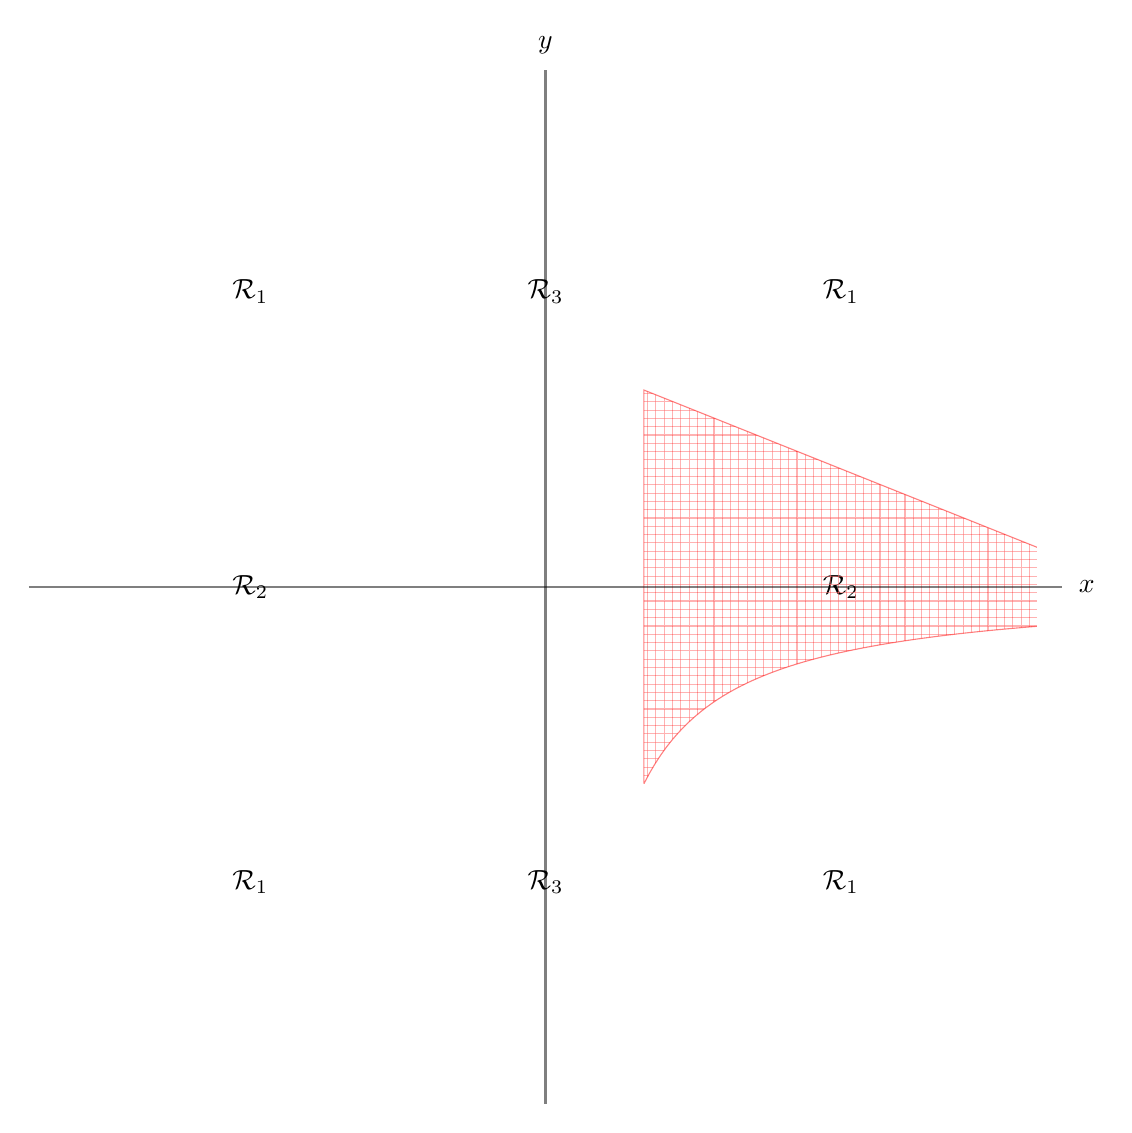
\begin{tikzpicture}[scale=1.25]
%Priming region
\draw[color=black,thick,fill=black!30,opacity=.5]	plot[id=Q1,domain=.2:5,samples=70]
function{1/(x)}--(5,.2)--(5,5)--(.2,5);
\draw[color=black,thick,fill=black!30,opacity=.5]	plot[id=Q4,domain=.2:5,samples=70]
function{-1/(x)}--(5,-.2)--(5,-5)--(.2,-5);
\draw[color=black,thick,fill=black!30,opacity=.5]	plot[id=Q3,domain=-5:-.2,samples=70]
function{1/(x)}--(-.2,-5)--(-5,-5)--(-5,-.2);
\draw[color=black,thick,fill=black!30,opacity=.5]	plot[id=Q2,domain=-5:-.2,samples=70]
function{-1/(x)}--(-2,5)--(-5,5)--(-5,.2);
\node at (3,3) {$\mathcal{R}_1$};
\node at (3,-3) {$\mathcal{R}_1$};
\node at (-3,-3) {$\mathcal{R}_1$};
\node at (-3,3) {$\mathcal{R}_1$};
\node at (3,0) {$\mathcal{R}_2$};
\node at (-3,0) {$\mathcal{R}_2$};
\node at (0,3) {$\mathcal{R}_3$};
\node at (0, -3) {$\mathcal{R}_3$};
\node at (0,5.5) {$y$};
\node at (5.5,0) {$x$};
%Top region
  \draw[color=blue,thin,pattern=crosshatch,pattern color=blue!60,opacity=.5,samples=70]
 plot[id=topRight,domain=.4:1] function{2/(x)}-- (2,1)--(-2,1)--
    plot[id=topLeft,domain=-1:-.4] function{-2/x};
%Bottom region
  \draw[color=blue,thin,pattern=crosshatch,pattern color=blue!60,opacity=.5,samples=70]
plot[id=bottomRight,domain=.4:1] function{-2/x}-- (2,-1)--(-2,-1)--plot[id=bottomLeft,domain=-1:-.4] function{2/x};
%Right region
   \draw[color=red,thin,pattern=grid,pattern color=red!60,opacity=.5,samples=70] 	(1,-2)--(1,2) -- plot[id=rightTop,domain=1:5] function{2/(x)}-- (5,.4)--(5,-.4)--
    plot[id=rightBottom,domain=1:5] (6-\x,{-2/(6-\x)});
%Left region
   \draw[color=red,thin,pattern=grid,pattern color=red!60,opacity=.5,samples=70] 	plot[id=leftBottom,domain=-5:-1] function{2/(x)}--(-1,-2)--(-1,2) --
    plot[id=leftTop,domain=-5:-1] (-6-\x,{-2/(-6-\x)});

%axes
\draw[color=white,thick] (5,5)--(5,-5)--(-5,-5)--(-5,5) --(5,5);
\draw[thick,color=black,opacity=.5] (-5.25,0) -- (5.25,0);
\draw[thick,color=black,opacity=.5] (0,-5.25) --(0,5.25);
\end{tikzpicture}
%\caption{Decomposition of plane into priming and diffusive regions.}
%\label{fig:regions}
%\caption{}
\end{figure}
\end{textblock}

\begin{textblock}{1}(36.25,24.7)
Figure 13
\end{textblock}


\begin{textblock}{5}(39.7, 20.2)
\begin{align*}
v_1(x,y) &= x^2 + y^2 \\
v_2(x,y) &= x^2+\frac{c_2^2}{x^2}+kc_2^2-kx^2y^2 \\
v_3(x,y) &= y^2+\frac{c_2^2}{y^2}+\tilde{k}c_2^2-\tilde{k}x^2y^2
\end{align*}
\end{textblock}



\begin{textblock}{11.5}(33.75,25)
\medskip
\LHead{\parbox{11.5in}{\begin{center}Conclusion\end{center}}}\\
\large
\begin{itemize}
\item In this project, we examined different Hamiltonian systems in order to investigate ways of perturbing them so that noise-induced stabilization can occur.
\item We systematically proved stability of the perturbed Hamiltonian systems by dividing the plane and finding local Lyapunov functions on each of these regions.
\item There are other Hamiltonian systems for which perturbations could allow for noise-induced stabilization.  Further work in this area could focus on developing techniques to identify and stabilize these systems.

\begin{comment}
\item We have analyzed the phenomenon of noise-induced stabilization, where the addition of noise to an unstable ODE has a stabilizing effect. We have proven the precise minimum noise necessary for stabilization when the drift and noise coefficients are general power functions, polynomials, or exponential or logarithmic functions.
\qquad\\
\item Future work could look at other forms for the drift and noise coefficients and explore the minimum amount of noise necessary to stabilize the ODE where the noise coefficient is not restricted to a specific form.
\end{comment}
\end{itemize}
\end{textblock}




\begin{textblock}{45}(-0.25,33.05)
\hspace{0in}
\hrule
\end{textblock}

\begin{textblock}{45}(-0.25,33.55)
\huge
\centering
Acknowledgements: \quad Valparaiso University \quad VERUM 2017 \quad National Science Foundation Award No.~1559912
\end{textblock}

\end{document}